\section{Introduction}
\label{netqasm:sec:introduction}

\dropcap{Q}uantum mechanics shows
that if one is able to communicate quantum information between nodes in a
network, one is able to achieve certain tasks which are impossible using only
classical communication. There are many applications~\cite{Wehner2018stages}
where a \emph{quantum network} has advantage over a \emph{classical
      (non-quantum) network}, either by (1) enabling something that is theoretically
impossible in a classical network, such as the establishment of an
unconditionally secure key~\cite{bb84} and secure blind quantum
computing~\cite{childs2005assisted} or (2) allowing something to be done faster
or more efficiently such as exponential savings in
communication~\cite{Buhrman2010} and extending the baseline of
telescopes~\cite{gottesman2012longer}. In recent years, many experiments have
been conducted to show that a quantum network is not only a theoretical concept,
and indeed advancements have been made to implement such a quantum network on
various hardware platforms. \cite{Hensen2015, Humphreys2018,
      moehring2007entanglement, hofmann2012heralded, Kalb2017, Inlek2017,
      sangouard2011quantum}. However, these experiments alone do not yet make a
quantum network \textit{programmable}, since the program logic was hard-coded
into the experimental hardware ahead of time. (There have been examples of
      experiments with some simple logic but only with a very limited number of
      pre-loaded decision-branches.)

% Before considering how to program quantum network applications, let us first
% briefly sketch the system our applications are run on. Abstractly, quantum
% networks consist of \textit{nodes} that are connected by \textit{channels}
% (\cref{background:fig:network_model}). Classical channels enable classical communication
% between nodes, while quantum channels are used for \textit{entanglement}
% generation between nodes. So-called \textit{end-nodes} may contain
% \textit{quantum processors} that can run arbitrary (quantum) programs. They have
% access to a quantum memory consisting of qubits, on which they can perform
% operations, including quantum computations. Some of these qubits may be used for
% establishing an entangled quantum state with a remote node. An end-node also
% possesses a classical processor and a classical memory. Furthermore, an end-node
% can send and receive classical messages to and from other end-nodes in the
% network. A network of quantum networks may be a called a \textit{quantum
%       internet}.

% Quantum (network) processors differ from classical processors in a number of
% ways. Firstly, quantum memory has limited lifetime, meaning that its quality
% degrades over time. For example, quantum memories based on nitrogen-vacancy (NV)
% centers in diamond have impressively been optimized to achieve lifetimes in the
% order of seconds~\cite{Abobeih2018}; however, this is still very short compared
% to classical memories, which generally do not have a limited lifetime at all.
% Therefore, the quality of program execution is time-sensitive. Secondly,
% physical devices are prone to inaccuracies which lead to decreased quality of
% (quantum) computation. For example, applying an operation (like a gate) on a
% qubit affects that qubit's quality. We note that the two challenges mentioned so
% far are also inherent to non-network quantum processors. Quantum
% \textit{network} processors have additional challenges: (1) the processor may
% have to act as a local computation unit and a network interface at the same
% time; for example, in NV centers, an electron spin qubit is used for generating
% entanglement with a remote node but is also needed to do local two-qubit gates,
% (2) remote-entanglement operations may not have a fixed time in which they
% complete, which makes scheduling and optimization more difficult.

% Quantum network \textit{applications}, also called \textit{protocols}, are
% multi-partite programs that involve entanglement generation and classical
% communication between different end-nodes, as well as local computation.
% Examples include Quantum Key Distribution (QKD)~\cite{bb84, ekert1991quantum},
% leader election protocols~\cite{kobayashi2014simpler, ganz2009quantum}, and
% Blind Quantum Computation (BQC)~\cite{Wehner2018stages}. Such applications are
% split into distinct \textit{programs} each of which runs on a separate end-node.
% The programs consist of both local operations (classical and quantum) and
% network operations (classical and quantum), see \cref{fig:app_programs}. That
% is, the programs communicate either by passing classical messages, or by
% establishing quantum entanglement. For example, BQC involves a \textit{client}
% node and a \textit{server} node, both of which run their own program. Their
% joint execution looks roughly as follows: (1) The client and server engage in
% remote entanglement generation such that the server's quantum memory ends up
% being in a certain state, (2) the client sends instructions to the server in the
% form of a classical message, (3) the server performs a measurement-based
% computation on its own quantum memory based on the client's instructions, (4)
% the server sends measurement results back to the client, (5) the client sends
% new instructions based on the measurement results, (6) repeat steps 3 to 5 until
% the client obtains its desired result.

% The example above illustrates that quantum network programs consist of different
% types of operations. Indeed, program code consists of \textit{classical code},
% containing local classical operations and classical communication with other
% nodes, and \textit{quantum code}, which are operations on quantum memory (such
% as \textit{gates}) and remote entanglement generation. Blocks of these types of
% code may depend on each other in multiple ways, as depicted
% in~\cref{fig:program_decomp}. Programs with mixed classical and quantum
% operations have also been called \textit{dynamic quantum
%       circuits}~\cite{cross2021openqasm, burgholzer2021towards}, but these do not
% cover the networking dimension found in programs we consider here, such as the
% dependency on remote information and entanglement generation operations.

% Due to the nature of quantum network programs, execution may have to
% \textit{wait} for some time. For example, the program needs to wait until
% another node sends a classical message, or until remote entanglement has been
% established. Therefore, it makes sense to run multiple (independent) quantum
% network programs on a node at the same time (interleaved), so that processor
% idle times can be filled by execution of other programs. This is something that
% typically does not happen on local quantum computers, and therefore introduces
% new challenges.

% Quantum network applications may be programmed by a single actor. For example, a
% developer may program a QKD application in the form of a two programs, and
% distribute these two programs to two end-nodes in the network. Alternatively, a
% single-node quantum network program may be developed separately from other
% programs, possibly not knowing how these other programs are implemented. For
% example, a BQC service provider could have already implemented the server-side
% program of a specific BQC protocol. A client may then write the client-side of
% this protocol, without having control over the server-side implementation.

The aim of this work is to propose a way to program quantum network programs
and execute them on the end-nodes of a quantum network.


\begin{figure}[t]
    \centering
    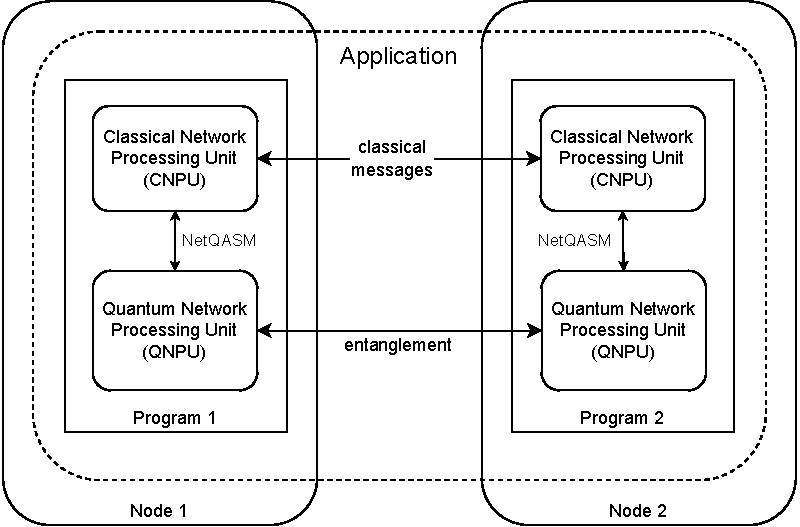
\includegraphics[width=0.6\linewidth]{figures/netqasm/multi_program_app_2.pdf}
    \caption{A quantum network application consists of a program for each of the nodes involved in the application.
        Each program is locally executed by the node.
        Program execution on each node is split into execution in an application layer, which can send and receive classical messages, and a quantum processor, which can create entanglement with another node.
        The communication between nodes can hence be both classical and quantum.
        Communication instructions need to be matched by corresponding instructions in the other program.
        There is no global actor overseeing execution of each of the programs, and the nodes may be physically far apart.}
    \label{fig:app_programs}
\end{figure}

\begin{figure}[t]
    \centering
    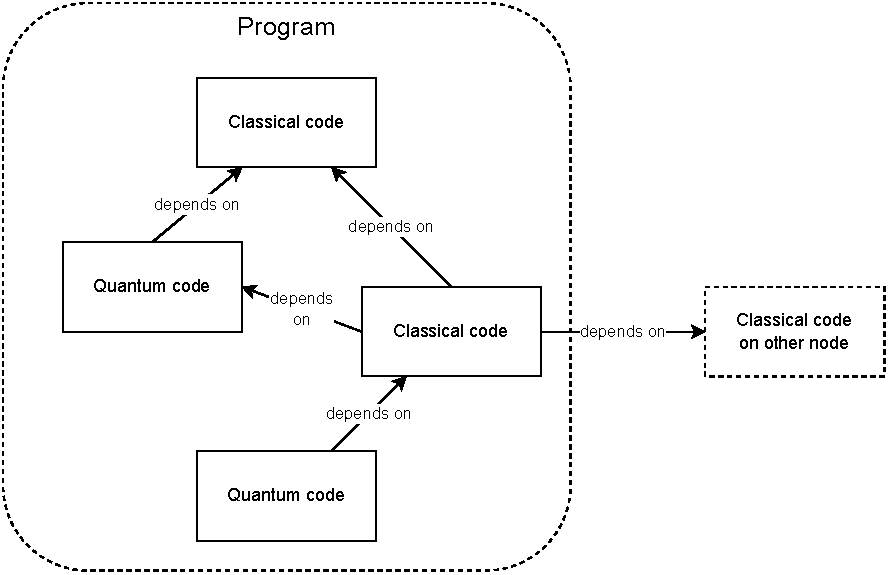
\includegraphics[width=0.6\linewidth]{figures/netqasm/program_decomp.pdf}
    \caption{A program on a single node consists of different blocks of code, which can be quantum (pure quantum instructions with classical control in between), or classical (no quantum operations at all).
        These blocks may depend on each other in various ways.
        For example, the outcome of a measurement happening in one of the quantum blocks may be used in a calculation performed in one of the classical blocks.
        Blocks may also depend on other nodes.
        For instance, the value of a message coming from another node can influence the branch taken in one of the classical blocks.}
    \label{fig:program_decomp}
\end{figure}


In this chapter we introduce an abstract model---including a \ac{QNPU}--- for end-nodes in a quantum network, which we define in \cref{netqasm:sec:abstract_model}.
We then propose \ac{NetQASM}, an instruction set architecture that can be used to run arbitrary programs (of the form described in \cref{fig:program_decomp}) on end-nodes, as long as the end-nodes realize the model including the QNPU.

\ac{NetQASM} consists of a specification of a low-level assembly-like language to express the quantum parts of quantum network program code.
It also specifies how the application layer should interact with the \ac{QNPU} and how the assembly language can be used to execute (network) quantum code.
This is not possible using other QASM languages.

The \ac{NetQASM} language is extendible using the concept of \textit{flavors}.
The core language definition consists of a common set of instructions that are shared by all flavors.
This common set contains classical instructions for control-flow and classical memory operations.
This allows the realization of low-level control logic close to the quantum hardware;
for example, to perform branching based on a measurement outcome.
Quantum-specific instructions are bundled in flavors.
We introduce a \textit{vanilla} flavor containing universal platform-independent quantum gates.
Using this flavor of the \ac{NetQASM} language enables the platform-independent description of quantum network programs.
Platform-\textit{specific} flavors may be created to have quantum operations that are native and optimized for a specific hardware platform.
As an example, we show a flavor tailored to the Nitrogen-Vacancy (NV) hardware, a promising platform for quantum network end-nodes~\cite{Taminiau2014, hanson2021realization}.

In our model, application-specific classical communication only happens at the application layer (\cref{fig:app_programs}).
In particular, this means that \ac{NetQASM} contains no provision for classical communication with the remote node.
We remark that of course, classical control communication may be used by the \ac{QNPU} to realize the services of the quantum network stack accessed through \ac{NetQASM}.

We note that \ac{NetQASM} is used for representing and running code that runs on a single node in a quantum network.
Synchronization between the (\ac{NetQASM}) programs of multiple nodes is the responsibility of the programmer.
For example, in a client-server application, if the client code contains a `receive classical message' operation, it is the responsibility of the server node that its program code contains a `send classical message' operation at the right moment.
The same holds for instructions for creating remote entanglement.
In terms of precise timing, which is needed for entanglement generation, it is the \ac{QNPU} that is responsible to communicate and synchronize with the \ac{QNPU} of the other node to make sure entanglement attempts are synchronized.

With \ac{NetQASM}, we solve various problems that are unique to quantum internet programming:
    (1) for remote entanglement generation, we introduce new instruction types for making use of an underlying quantum network stack~\cite{dahlberg2019linklayer, kozlowski2020networklayer},
    (2) for the close interaction between classical and quantum operations, we use a shared-memory model for sharing classical data between the application layer and the \ac{QNPU},
    (3) in order to run multiple applications on the same quantum node---which may be beneficial for overall resource usage (see~\cref{netqasm:sec:design_considerations})---we make use of virtualized quantum memory, similar to virtual memory in classical computing~\cite{arpaci2018operating},
    (4) since on some platforms, not all qubits may be used to generate remote entanglement, we introduce the concept of unit-modules describing qubit topologies with additional information per (virtual) qubit about which operations are possible.

Since \ac{NetQASM} is meant to be low-level, similar in nature to classical assembly languages, we have also developed a higher-level software development kit (SDK), in Python, to make it easier to write applications.
This SDK and related tools are open-source and freely available at~\cite{git_netqasm}, as part of our Quantum Network Explorer~\cite{qne_website}.
Through the SDK we have also enabled the quantum network simulators NetSquid~\cite{coopmans2021netsquid} and SimulaQron~\cite{dahlberg2018simulaqron} to run any application programmed in \ac{NetQASM}.

We have evaluated \ac{NetQASM} by simulating the execution of a teleportation application and a blind quantum computation using \ac{NetQASM}.
Hereby we have shown that interesting quantum internet applications can indeed be programmed using \ac{NetQASM}.
Furthermore, the evaluations argue certain design choices of \ac{NetQASM}, namely the use of so-called \textit{unit modules}, as well as platform-specific
\textit{flavors}.

We remark that \ac{NetQASM} has already been used on a real hardware setup in the lab, in a highly simplified test case that only produces entanglement~\cite{pompili2021experimental}.
Furthermore, in \cref{chp:qnodeos}, we present a full stack implementation that uses \ac{NetQASM}.


\subsection{Related Work}
\label{netqasm:sec:related}

% \todo{Remove parts that are already in Background chapter and just refer to them}
In the field of quantum computing, a substantial amount of progress has been made related to developing
architectures (e.g.~\cite{fu2017microarchitecture,bourassa2020photonicblueprint, murali2019fullstack, wecker2014liqui, khammassi2020openql, amy2019staq, green2013quipper, Steiger2016}),
instruction sets (e.g.~\cite{cross2017openqasm,khammassi2018cqasm,fu2019eqasm,liu2017fqasm,smith2016quil,qiskit,cirq,qsharp,jones2019quest}) and
compilers~\cite{zulehner2019compiling, haner2018software, gokhale2020quantum, liu2020new, gokhale2020optimized, ding2020square, smith2020opensource, Sivarajah_2020, hietala2019verified, zhang2020contextmapping, niu2020hardware, dury2020qubo, pozzi2020using, Nishio_2020}.
One example is QASM, an instruction set framework, borrowing ideas from classical assembly languages, which has gained a lot of popularity over the years and has been successfully integrated in software stacks for quantum computers.
There are in fact many variants of QASM such as OpenQASM~\cite{cross2017openqasm}, \texttt{cQASM}~\cite{khammassi2018cqasm}, \texttt{eQASM}~\cite{fu2019eqasm}, \texttt{f-QASM}~\cite{liu2017fqasm}.
Some of these variants are at a level closer to the physical implementation, such as \texttt{eQASM}, allowing for specifying low-level timing of quantum operations, while others, such as \texttt{f-QASM}, are at a higher level.
Together with the definition of these QASM-variants, progress has also been made in compilation of applications programmed in QASM to hardware implementations.
More abstract languages and programming frameworks for quantum programs include \texttt{Quil}~\cite{smith2016quil}, \texttt{Qiskit}~\cite{qiskit}, \texttt{Cirq}~\cite{cirq}, \texttt{Q\#}~\cite{qsharp}, \texttt{QuEST}~\cite{jones2019quest}.

None of these instruction sets or languages contain elements for remote entanglement generation (i.e. between different nodes), which \ac{NetQASM} does provide.
A \ac{NetQASM} program that uses the vanilla flavor and only contains local operations would look similar to an OpenQASM program.
However, the instruction set is not quite the same, since \ac{NetQASM} uses a different memory model than OpenQASM.
This is due to the hybrid nature of quantum network programs, which has more interaction between classical data and quantum data than non-networking programs (for which OpenQASM might be used).
So, \ac{NetQASM} is not just a superset of the OpenQASM instruction set (in the sense of adding entanglement instructions).

In~\cite{dahlberg2018simulaqron}, we introduced the \ac{CQC} interface, which was a first step towards a universal instruction set.
However, \ac{CQC} had a number of drawbacks, in particular:
    (1) \ac{CQC} does not have a notion of virtualized memory (see \cref{netqasm:sec:design_considerations}), which meant that applications needed to use qubit IDs that were explicitly provided by the underlying hardware.
        This introduced more communication overhead and fewer optimization opportunities for the compiler.
    (2) \ac{CQC} does not provide as much information about hardware details.
        Therefore, platform-specific compilation and optimization is not possible.
    (3) Furthermore, \ac{CQC} does not match entirely with the later definition of our quantum network stack~\cite{dahlberg2019linklayer, kozlowski2020networklayer}.
        For example, it was not clearly defined how \ac{CQC} relates to the definition of a network layer.

Many of the ideas from e.g. QASM for how to handle and compile local gates can be reused also for quantum network applications.
For example, version 3 of OpenQASM~\cite{cross2021openqasm} which is under development, proposes close integration between \emph{local} classical logic and quantum operations, which is something we also propose in this work.
However, there are two key differences that we need to address:
\begin{enumerate}
      \item Instructions for generating entanglement between remote nodes in the network need to be handled and integrated with the rest of the application, see \cref{netqasm:sec:abstract_model} below.
      \item The local operations performed by a node might depend on information communicated by another node and only known at runtime.
            Note that this is different from the conditionals on \emph{local} classical information, proposed in for example OpenQASM version 3, which does not require communication between remote nodes in a network.
            This brings new constraints in how to handle memory allocation, scheduling and addressing.
            We discuss this point in further detail in the coming sections.
\end{enumerate}
\ac{NetQASM} solves the above two points and improves upon \ac{CQC}.


\subsection{Outline}
In \cref{netqasm:sec:abstract_model} we define relevant concepts and introduce the model of end-nodes that we use, including the \ac{QNPU}.
In \cref{netqasm:sec:use_cases} we discuss use-cases of a quantum network which \ac{NetQASM} should support.
In \cref{netqasm:sec:design_considerations} we consider requirements and considerations any instruction set architecture for quantum networks should fulfill which then lay the basis for the decisions that went into developing \ac{NetQASM}, see \cref{netqasm:sec:design_decisions}.
In \cref{netqasm:sec:implementation} and \cref{netqasm:sec:python-sdk} we describe details about the \ac{NetQASM} language and associated SDK.
In \cref{netqasm:sec:evaluation} we quantitatively evaluate some of the design decision of \ac{NetQASM} by benchmarking quality of execution using the quantum network simulator NetSquid~\cite{netsquid,coopmans2021netsquid}.
We conclude in \cref{netqasm:sec:conclusion}.